\chapter{Objectives and information in data}
\thispagestyle{fancy}
\label{ch:objectives-and-information-in-data}



\hrule
\begin{itemize}
\footnotesize
\item[]{Aims:}
\begin{enumerate}
\item{to be aware of the added value of carefully interpreting the results of
the parameter evolution;}
\item{to understand the effect of noise in the measurements;}
\item{to understand the effect of the distribution of observations in relation
to the model's local sensitivity (or system behavior);}
\item{to experience the added value of data transformations for parameter
identification;}
\item{to understand the consequences of model structural errors for the
parameter optimization process and result;}
\item{to experience the opportunities of multi-objective optimization.}
\end{enumerate}
\end{itemize}
\hrule
\vspace{1em}


Often people perform a model calibration, then they present the final model
result, and then\ldots they are done. But in fact the most interesting part of
inverse modeling is the interpretation of both the results of the evolution of
the parameter search and of the simulation results. In this chapter, we will
investigate the relation between model complexity, measurement error, and the
type of observations.

\section{Case: cubic model}

\smallq{Use the MATLAB editor to open `dreamWithCubicmodel.m' located in
`./exercise/dream-cubicmodel/'. After briefly studying the program, press F5 to
run it as provided with 14 data points (variables \mcode{xObs} and
\mcode{yObsNoisy}). Don't forget to save the results (check the code snippet on
page~\pageref{lst:save-print} or copy and paste in a PowerPoint presentation).}

\smallq{To identify the parameters of a 4-parameter model, 14 data points aren't
very many. How do you think the results will change if you increase the number
of data points? Check your hypothesis by setting \mcode{xObsStep} to 0.2.}

\smallq{Not only the number of the data points is important, but also the
distribution. Argue what would be the result if you wouldn't have had the data
points below x=3 (keep \mcode{xObsStep} at 0.2). Explain which parameters you
expect to be identified most accurately? Then check whether your hypothesis was
correct.}

\smallq{If you could do one more measurement between x=-1 and x=7, where would
you place it? Explain why.}

\smallq{What if you would have only the observations below x=3 (keep
\mcode{xObsStep} at 0.2)? Again, explain which parameters you expect to be
identified most precisely and then check whether your hypothesis was correct.}

\smallqo{If you would increase the magnitude of the error term
(\mcode{gaussTerm}), how will that affect the results? Check your hypothesis by
making the appropriate changes to the script.}

\section{Case: rainfall interception}

In this part, we will interpret the relation between data, model and selected
parameters using a simplified version of an existing rainfall interception model
\citep{bout-scha-aert-verm1996}. This version simulates canopy water storage
using one layer only. As with any model, it is important that you understand
both the concept of the model---including equations, parameters and boundary
conditions---as well as the measurements used in the inverse modeling; if you
don't, it is impossible to interpret the results.

Conceptually, the interception model is a very simple water balance of the
canopy. Water storage in the canopy (S) changes with time $t$, as a result of
precipitation (P), interception (I), drainage (D) and evaporation (E); see
Figure~\ref{fig:interception-model-flows} and
Equation~\ref{eq:interception-model}.
\begin{equation}
\label{eq:interception-model}
\frac{\Delta S}{\Delta t} = I-D-E
\end{equation}
\begin{tabular}{lll}
with:&&\\
$S$&canopy water storage&\textsf{mm}\\
$t$&time&\textsf{day}\\
$I$&interception rate&\textsf{mm$\cdot{}$day$^{-1}$}\\
$D$&canopy drainage rate&\textsf{mm$\cdot{}$day$^{-1}$}\\
$E$&canopy evaporation rate&\textsf{mm$\cdot{}$day$^{-1}$}\\
\end{tabular}

\begin{figure}[htbp]
  \centering
    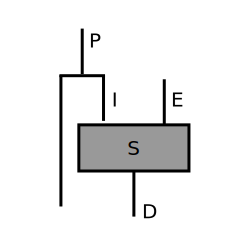
\includegraphics[width=0.3\textwidth]{./eps/converted/interceptionmodel-flows}
  \caption{Definition of flows for the interception model.}
  \label{fig:interception-model-flows}
\end{figure}

\needspace{5\baselineskip}Precipitation and potential evaporation ($E_0$) are
the measured boundary conditions. The other fluxes are calculated as:
\begin{equation}
I=a\cdot{}P
\end{equation}
\begin{equation}
D =
\begin{cases}
b\cdot{}(S-c), & \text{if }S>c\\
0, & \text{if }S\leq{}c\\
\end{cases}
\end{equation}
\begin{equation}
E = d\cdot{}E_0\cdot{}\frac{S}{c}
\end{equation}
\begin{tabular}{lll}
{\bf parameter}&{\bf description}&{\bf units}\\
$a$&interception efficiency (canopy cover fraction)&\textsf{-}\\
$b$&canopy drainage efficiency&\textsf{day$^{-1}$}\\
$c$&canopy water storage capacity&\textsf{mm}\\
$d$&evaporation efficiency&\textsf{-}\\
\end{tabular}



Before optimizing the model parameters $a$, $b$, $c$ and $d$, you need to get a
better understanding of the meaning of each parameter, and its effect on the
model prediction. With this knowledge you will be able to choose a more
meaningful minimum and maximum parameter space and your optimization will
converge faster.

\smallq{Use the MATLAB editor to open `mancal\_interceptionmodel' located in
`./exercises/manual-calibration-interception-model/'. After pressing F5 to run
the script, a graphical user interface (GUI) will appear. If you run the model
with the input values $a$ = 0.6, $b$ = 200, $c$ = 2.5 and $d$ = 0.83, you will
get a plot similar to those in  Figure~\ref{fig:interceptionmodel-mancal-gui}.
Explain the output of this simulation:

\begin{itemize}
\item{why does the storage increase at $t$ = 0.75?}
\item{why does it reach a constant level?}
\item{why is this level 2.6?}
\item{why does this level change at $t$ = 1.0?}
\item{why does this level become 2.5?}
\item{why does the storage decrease at $t$ = 1.25?}
\item{explain the shape of the storage curve after $t$ = 1.25.}
\item{draw the canopy evaporation rate in
Figure~\ref{fig:interceptionmodel-mancal-gui}.}
\end{itemize}
}% smallq

\begin{sidewaysfigure}
%\begin{figure}[htbp]
  \centering
    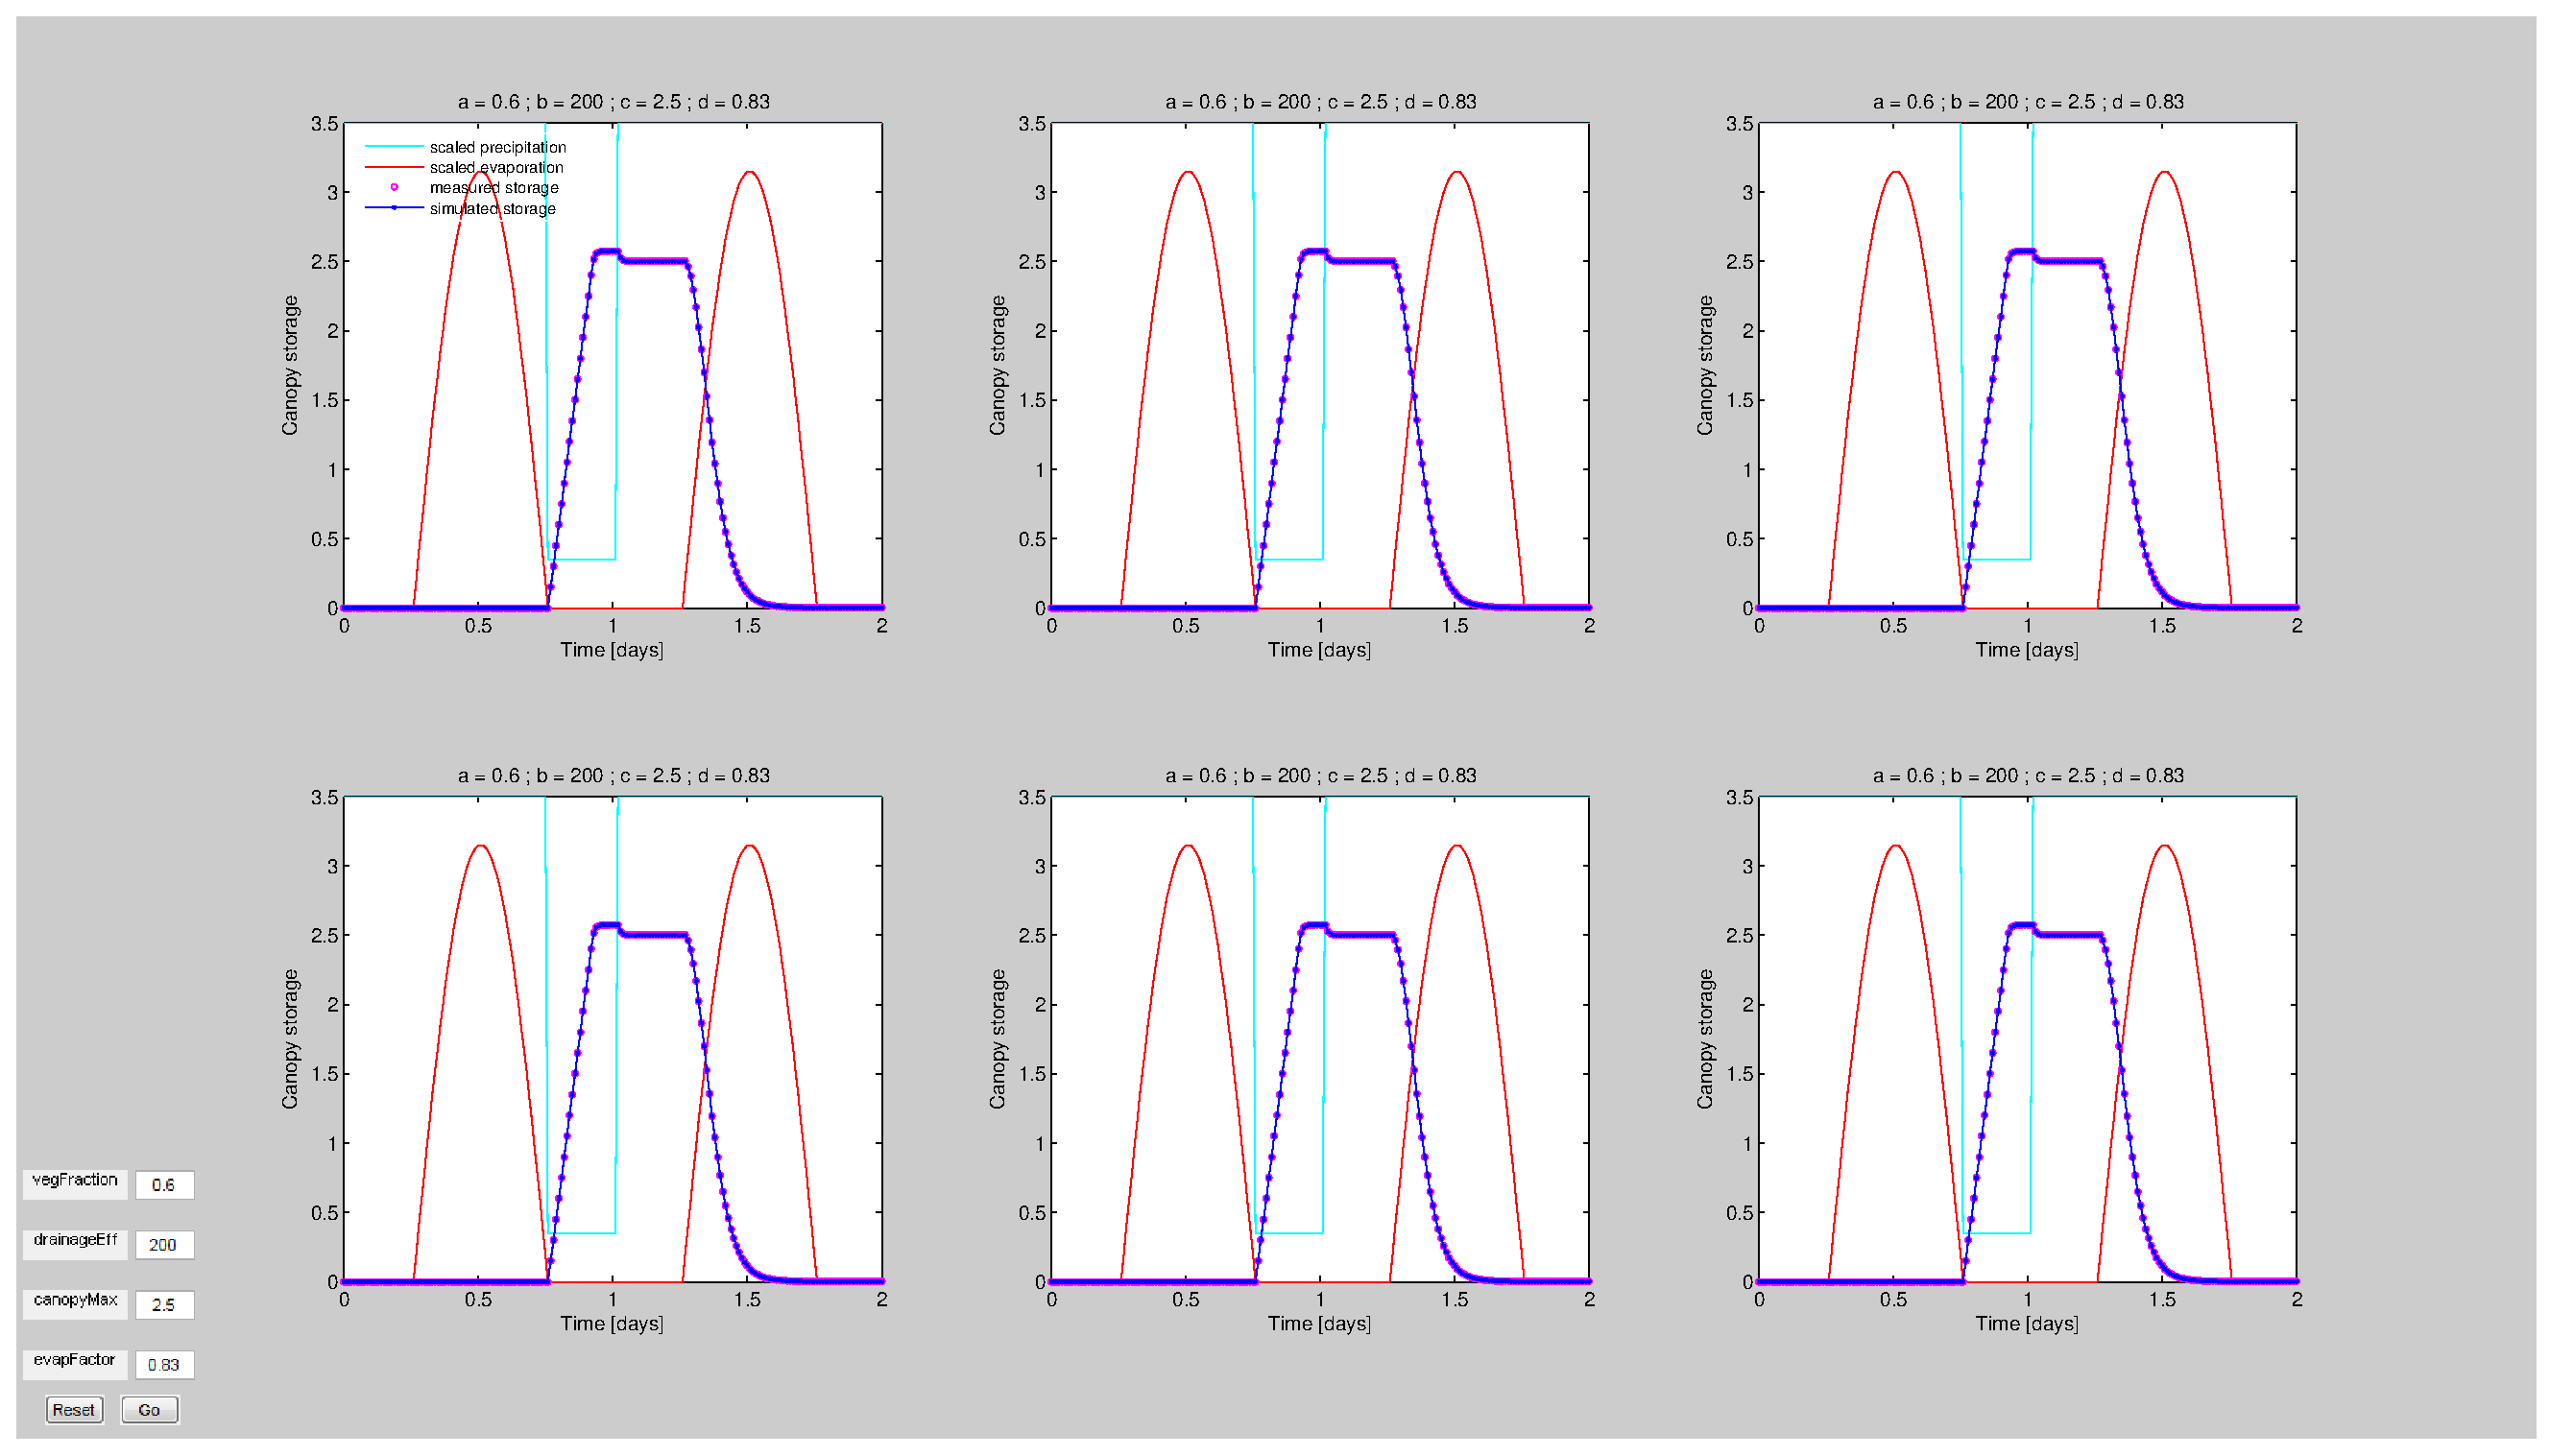
\includegraphics[width=1.0\textheight]{./eps/converted/interceptionmodel-mancal-gui}
  \caption{Graphical user interface showing the model prediction for $a$ = 0.6,
$b$ = 200, $c$ = 2.5 and $d$ = 0.83, based on simplified boundary conditions.}
  \label{fig:interceptionmodel-mancal-gui}
%\end{figure}
\end{sidewaysfigure}

\smallq{Next we will alter the parameter values only one at a time (!) and
predict how the change affects the model result. So, choose a parameter, then
first draw your prediction in one of the subplots of
Figure~\ref{fig:interceptionmodel-mancal-gui}. Only after you've drawn your
prediction, change the parameter value in the GUI. Press the `Go' button to run
the interception model with the changed parameter. Try to explain why your
prediction diverges from the model result. This is a useful procedure to better
understand the behavior of a system.}

\smallq{Summarize the knowledge you gained about each parameter's effect on the
model result.}

\subsection{Distribution of information within the data}

Having done the manual calibration, you are ready to interpret the results of
the interception model with boundary conditions that are more realistic. In the
next few exercises, we will perform several DREAM calibrations of the
interception model using  different data sets.

As a first step, it is always wise to first check your inverse modeling design
with so-called `artificial measurements'. Artificial measurements are generated
by running the model with a known parameter set. Subsequent calibration of the
model to the artificial measurements should yield this same parameter set again.

\smallq{Use the MATLAB editor to open `dreamWithInterc.m' located in
`./exercises/dream-interception-model/'. By default this script uses the
simplified boundary condition that we used in the manual calibration. Run the
main script to check if the true parameters are found.}

\smallq{Now adapt your script to let it use the more realistic boundary
conditions, by uncommenting the appropriate parts in the script. Experiment with
different boundary conditions. Can you explain the differences between the
various data sets? And what is the difference between the realistic boundary
conditions on the one hand and the ideal case on the other?}

It is often interesting to calibrate your model parameters based on a subset of
the data. This way, you can get some idea of the type of information that is
needed to identify each model parameter with precision and accuracy. The generic
way to have DREAM use subsets, is by adding a field to \mcode{Extra} that
contains the observation times that you want to use as part of your objective
function:
\lstinputlisting[numbers=none,nolol,label={lst:subsetting-t-less-than-one}]{./../m/subsetting-t-less-than-one.m}
\needspace{3\baselineskip}Inside \mcode{interceptionmodel}, you can use the time
information to only export simulated storage values at the times specified in
\mcode{tObj}:
\lstinputlisting[numbers=none,nolol,label={lst:subsetting-modelside}]{./../m/subsetting-modelside.m}
\mcode{output} can subsequently be returned as the function's output argument,
after which DREAM will compare it to the contents of
\mcode{Measurement.MeasData}.

\needspace{15\baselineskip}After the optimization finishes, the script probably
throws an error in the visualization part. This is because the simulated time
series of storage now has less elements than \mcode{bounds(:,1)}. You can avoid
this by re-defining \mcode{Extra.tObj} just before re-running the last 1000
parameter sets:
\lstinputlisting[numbers=none,nolol,label={lst:subsetting-redefine-extra}]{./../m/interceptionmodel-subsets-redefine-extra.tobj.m}

\smallq{Adapt your script to let it use only the observations for which $t<1$
(simplified boundary conditions). Make sure that the storage values returned by
\mcode{interceptionmodel} refer to the times at which storage was observed. What
do you expect with regard to the identifiability of the parameters? Store the
results to be able to refer back to them later, for instance by copying and
pasting into a PowerPoint presentation.}

\smallq{\needspace{5\baselineskip}In the previous exercises, we have calibrated
to a time-based subset of the observations. However, you can also make a subset
based on certain characteristics of the data. For instance, make a subset based
on $S>2.2$~\textsf{mm} (use the `211' data), calibrate the interception model
and explain the results. Remember, you can add fields to \mcode{Extra} with
information you need inside your model's workspace. For instance, you could do:
\lstinputlisting[numbers=none,nolol,label={lst:subsetting}]{./../m/subsetting.m} } 

\smallq{If you didn't already do this, adapt the script such that the simulated
canopy storage dynamics are visualized starting from t=211.41 through t=212.65.
Let your visualization differentiate between observations that are part of the
objective set and those that aren't. You should get a figure more or less like
Figure~\ref{fig:interception-model-subsets}.
\begin{figure}[htbp]
  \centering
    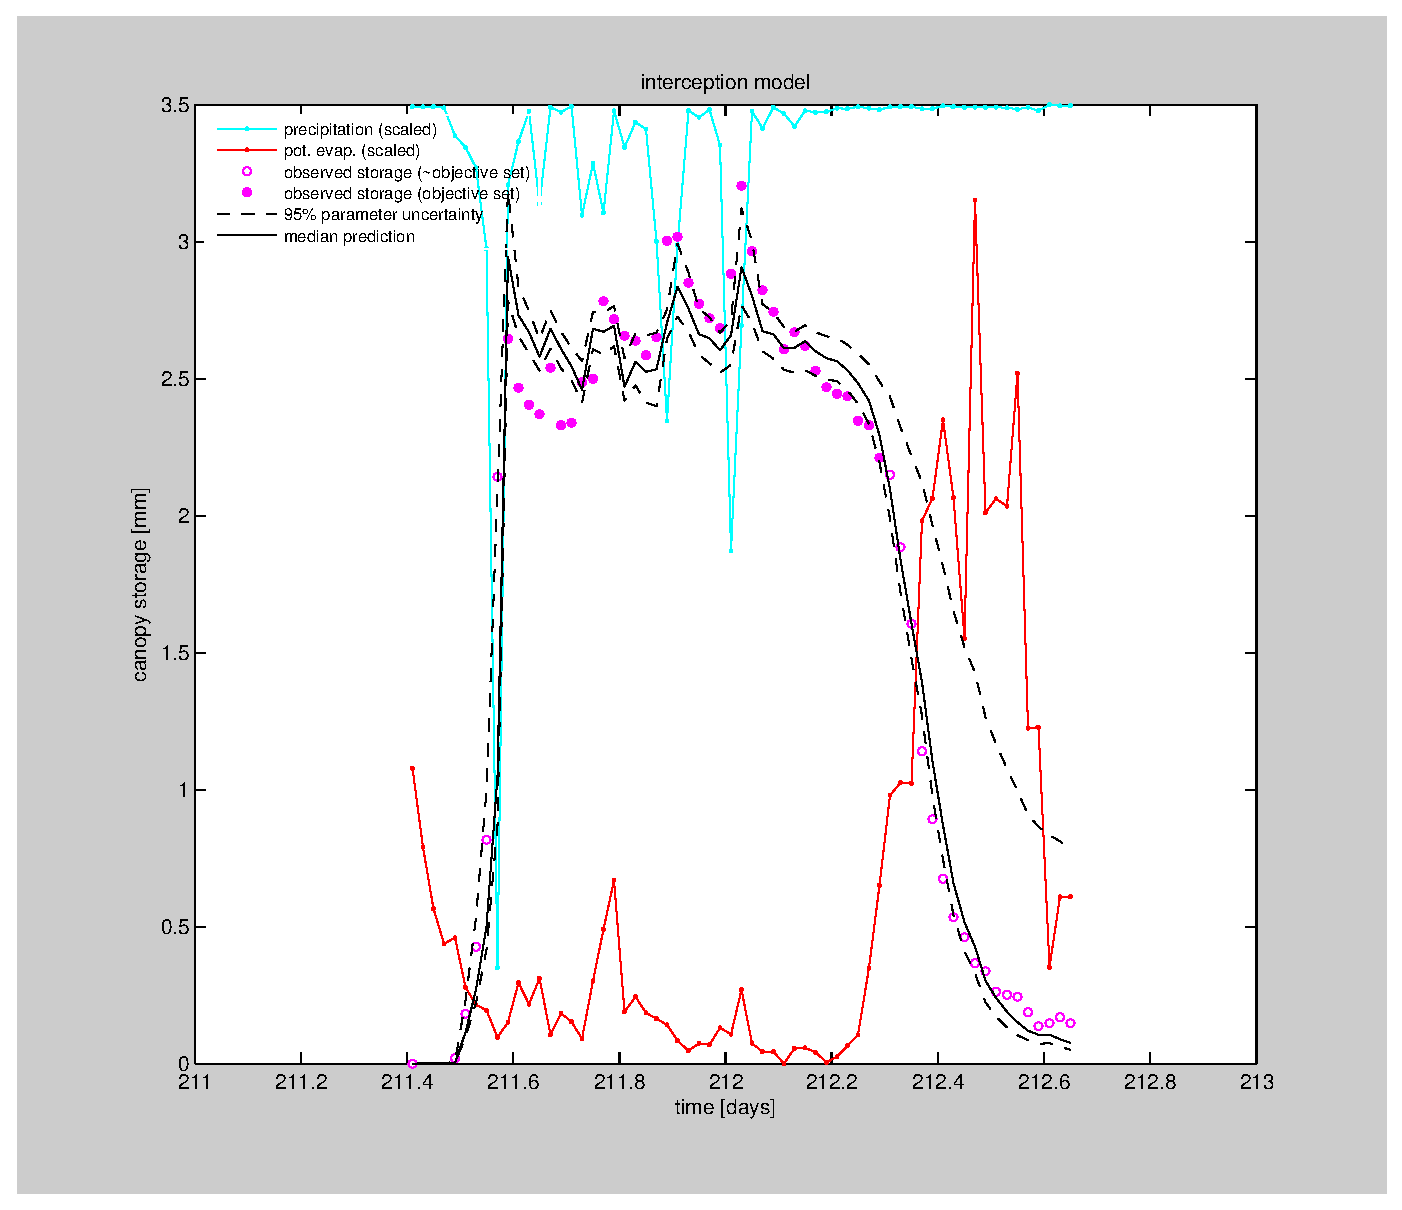
\includegraphics[width=1.0\textwidth]{./eps/converted/interceptionmodel-subset}
  \caption{Example of the interception model with objective based on high-storage
values only.}
  \label{fig:interception-model-subsets}
\end{figure}
}% smallq

\smallq{Describe the characteristics of a minimal data set with which the
parameters of the interception model can still be identified. Does the
measurement accuracy affect the minimal set?}


\subsection{Data transformations}

In this part, we will experiment with using different kinds of transformations.
For instance, squaring the observed data ($Y^2$) emphasizes the high values,
whereas $\sqrt{Y}$ and Box-Cox transforms ($\frac{Y^\lambda-1}{\lambda},
\lambda=0.3$) give more weight to lower (non-negative) values. Also, Box-Cox
transformations are often used when the error is known to be heteroscedastic
(i.e.~when the magnitude of the error is dependent on measurement value).
$log(Y)$ and $log_{10}(Y)$ should be avoided if Y-values of 0 can occur.

\smallq{Use the MATLAB editor to open `dreamWithHymodBoxCox.m' located in
`./exercises/dream-hymod-box-cox'. Despite its name, the script does not perform
a Box-Cox transform yet, but we'll get to that in a minute. First run the script
as provided and interpret the results.}

\smallq{What change in model performance or identifiability of parameters would
you expect if you apply the Box-Cox transform? Before running the script, we
need to make some small changes first. Of course, you need to transform the
observations as well as the model output. In order to  visualize the
optimization results, we need to adapt the model such that it can output either
the untransformed simulated storage or the transformed simulated storage,
depending on a flag \mcode{Extra.argOutIsTransformed} which can be \mcode{true}
or \mcode{false}. For instance:
\lstinputlisting[numbers=none,nolol,label={lst:argOutIsTransformed-modelside}]{./../m/argOutIsTransformed-modelside.m}
This is an easy way to use transformed data for the optimization, and
untransformed data for the subsequent visualization. Make the appropriate
changes in the program and check the answer you gave earlier.}

Another interesting transform is to use the derivative of the observations. This
can be particularly helpful with determining rates with respect to time.

\smallqo{What result do you expect if you apply the derivative transformation in
case of the cubic model?}

\smallq{Use the MATLAB editor to open `dreamWithIntercDerivative.m' located at
`./exercises/dream-interceptionmodel-derivative/'. As you can see, the objective
function operates on the derivative of storage. How do you think the prediction
will be different from the earlier results? Check your answer by running the
script.}



\section{Case: Easter Island population dynamics}


In the past few exercises we have seen that successful parameter identification
depends on what we call ``the information content of data''. It depends on:
\begin{enumerate}
\item{the signal/noise ratio (the higher the ratio, the faster the convergence
of the search procedure);}
\item{the sensitivity of the model for the parameters;}
\item{the distribution of the measurements in relation to this sensitivity.}
\end{enumerate}

Keep in mind that a model is never perfect and that deviations between model
output and observations is not by definition a Gaussian distribution. If the
model structure causes systematic errors, the inverse modeling procedure as used
until now will lead to a best fit while tuning the parameters. In this case the
optimal parameter values will compensate for the model structure error. In such
a case parameter identification produces the ``wrong'' (but optimal) parameter
values and convergence will also become slower.

To explore this effect in more detail, we will test a model of human population
and resources (trees/biomass) of Easter Island in the period 0-2000 AD. The
model is based on \citeauthor*{bran-tayl1998}~(\citeyear{bran-tayl1998}). The
governing equations and probable parameter values are as follows.

\needspace{15\baselineskip}

Rate of change of population:
\begin{equation}
\frac{dP}{dt} = (b+cr\cdot{}\frac{C}{P})\cdot{}P-(d-cr\cdot{}\frac{C}{P})\cdot{P}
\end{equation}
Rate of change of resources:
\begin{equation}
\frac{dR}{dt} = g\cdot{}(1-\frac{R}{Cc})\cdot{}R-C
\end{equation}
Consumption rate:
\begin{equation}
C = p\cdot{}P\cdot{}R
\end{equation}

\begin{tabular}{llll}
with:&&&\\
&\textbf{variable name as used}&\textbf{description}&\textbf{probable value}\\
&\textbf{in the model}&&\\
$P$&\mcode{Pop}&human population&\\
$R$&\mcode{Res}&resources (biomass)&\\
$b$&\mcode{parPopGrowth}&relative birth rate&0.02\\
$d$&\mcode{parDeathRate}&relative death rate&0.03\\
$Cc$&\mcode{parCarCap}&carrying capacity&160\\
$cr$&\mcode{parConsResponse}&consumption response&150\\
$g$&\mcode{parRelResGrowth}&relative growth rate of resources&0.004\\
$cr\cdot{}\frac{C}{P}$&\mcode{consProfit}&consumption profit&\\
$p$&\mcode{parFit}&labor efficiency constant&0--1e-6\\
\end{tabular}


\smallq{\needspace{15\baselineskip}Use the MATLAB editor to open
`dreamWithEasterModel.m' from `./exercises/dream-easter-island/'.
Figure~\ref{fig:pop-res-figures} shows 5 data sets that we have created using
the model described above. Experiment with calibrating the \mcode{eastermodel}
based on either population or resources data from any of the files listed below.
Assume an initial Population of 20, and an initial Resources value of 160. To
help the interpretation of the results, here are a few pointers on how the data
were created:
\begin{enumerate}
\item{`pop-res-data-ref.mat' is the reference file that contains the artificial
observations generated with the parameters mentioned above, with only very
little noise superimposed;}
\item{`pop-res-data-ref-noise.mat' is the same as (1), but with more noise;}
\item{`pop-res-data-variable-deathrate.mat' is a file that contains the
artificial observations generated with the parameters mentioned above, except
that the death rate parameter was changed to 0.035 for $t>700$. Because the
\mcode{eastermodel} does not incorporate this change, a structural error is
present in the model. Also, there's only very little noise superimposed;}
\item{`pop-res-data-variable-deathrate-noise.mat' is the same as (3), but with
more noise.}
\item{`pop-res-data-high-deathrate.mat' is the same as (1), but with
\mcode{parDeathRate=0.035}.}
\end{enumerate}
}


\smallq{Explain the high correlation between \mcode{parDeathRate} and
\mcode{parPopGrowth} in the results of the calibration.}

\smallq{What is the effect of the higher noise in the observations?}

\smallq{Set the value of \mcode{parPopGrowth} to 0.02 (i.e.~exclude it from the
optimization) to avoid the high correlation between \mcode{parDeathRate} and
\mcode{parPopGrowth}. How do you think this will affect the optimization process
and the accuracy of the optimized parameters (in comparison to the former case)?
Evaluate the result. Is this what you expected? If not, explain the difference.}

\smallqo{If you want to play with this some more, you can make your own
artificial data using `eastermodelArtifMeas.m'.} 

\begin{figure}[htbp]
  \centering
    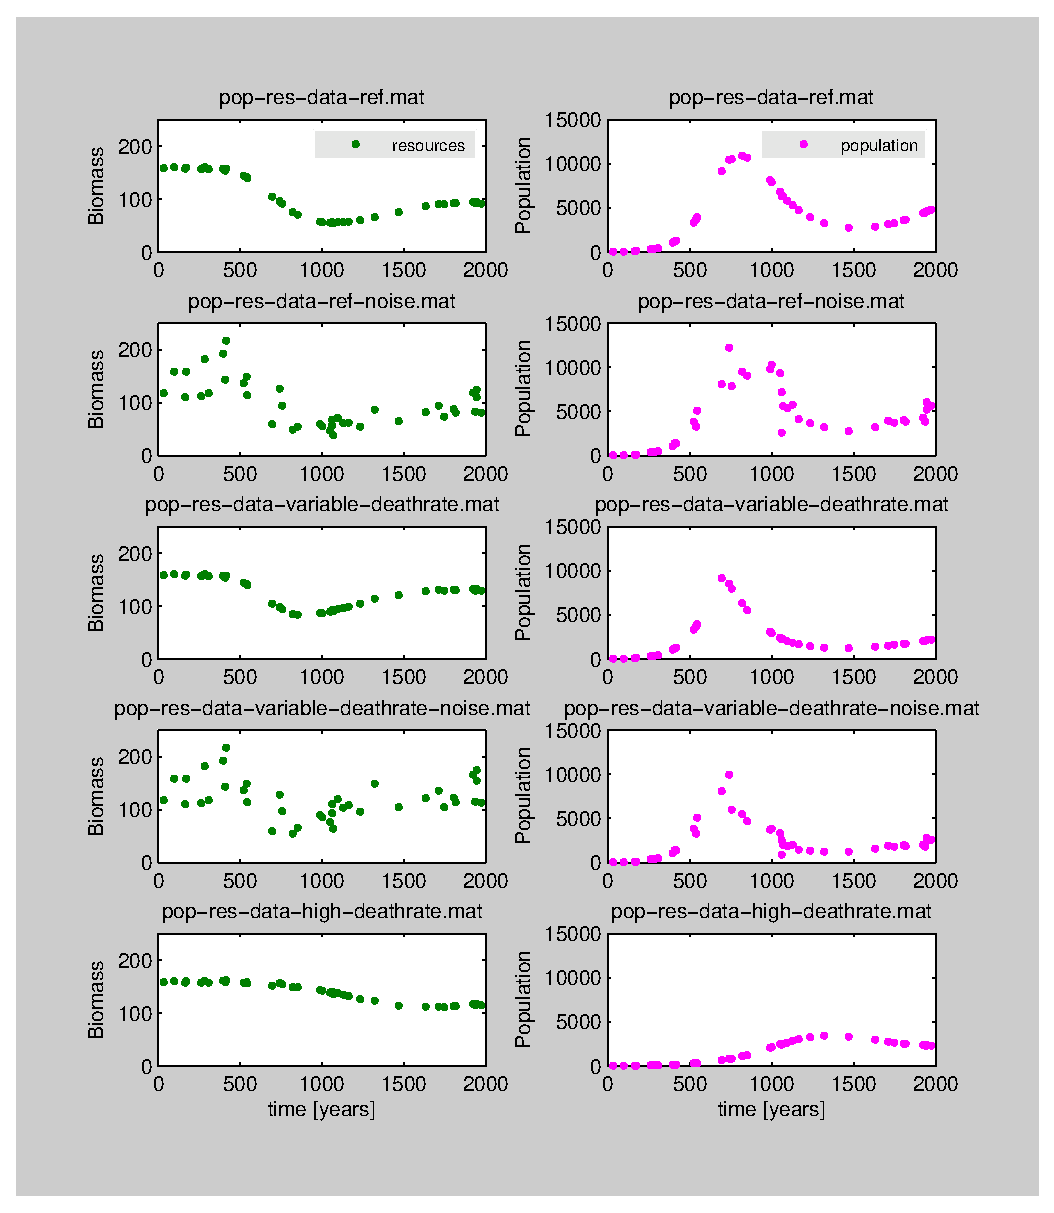
\includegraphics[width=1.0\textwidth]{./eps/converted/pop-res-figures}
  \caption{Resources-Population plots for the various files.}
  \label{fig:pop-res-figures}
\end{figure}



\needspace{15\baselineskip}

So far, we have calibrated the \mcode{eastermodel} based on either Population or
Resources, but you could also use both variables simultaneously. To do this, we
need to make some changes to the model:

\lstinputlisting[numbers=none,nolol,label={lst:weighted-error-series-modelside}]{./../m/weighted-error-series-modelside.m}

With this code, the model returns an error series, rather than the states
themselves, so the objective function should no longer compare model output with
observations; instead, we now want to minimize the model output. A simple way to
accomplish this is by setting \mcode{Measurement.MeasData} to
\mcode{zeros(size(PopMeas))}.

\smallq{Use the MATLAB editor to open `dreamWithEasterModelMO.m' from
`./exercises/dream-easter-island-mo/'. Make the appropriate changes to the
program in order to use both Population and Resources information. Set
\mcode{Extra.popWeight} to 1.0 for now (i.e.~ignoring the misfit on Resources)
and don't forget to initialize \mcode{Extra.argOutIsErr} as well. With this
weighting factor, your result should be similar to that of a single-objective
optimization (when the objective function operates on Population). Run the
script. Store your results.}

\smallq{Now do the same thing, but with all weight on the Resources. Again,
store the result.}

\smallq{Repeat one more time, but with half the weight on the Population and
half the weight on Resources. Store the result. Explain why the last result
looks much more like the result of \mcode{Extra.popWeight=1.0} than that of
\mcode{Extra.popWeight=0.0}.}

\smallq{How would you make sure that Population and Resources are treated as
equally important variables when \mcode{Extra.popWeight=0.5}? Implement your
solution and check if there is any difference with your earlier results.}

\smallq{Adapt the script to let it use the Resources data from
`pop-res-data-ref.mat' and the Population data from
`pop-res-data-high-deathrate.mat' with:
\lstinputlisting[numbers=none,nolol,label={lst:load-selected-variables}]{./../m/load-selected-variables.m}
Run the script for \mcode{Extra.popWeight} equal to 1.0, 0.0, and 0.5. Explain
the results. }%smallq



\smallqo{Looking back at the single-objective exercises that we have done
earlier this week, which one do you think would benefit from a multi-objective
approach? Explain what variables you would use in the calibration and which
objectives you would use (and why) before implementing it.}

\section{Multi-objective optimization of HYMOD}

\smallqo{In the directory `./exercises/hymod-so/' you will find the files to
apply the SCE-UA algorithm \citep{duan-gupt-soro1992} to the HYMOD model. We use
the same data as in previous exercises (Leaf River, Mississippi), and we analyze
the data from a single year (1953). Open `CompOF.m' and verify what objective
function is being used in the current optimization. In a first step, compare the
root mean square error (RMSE) and the mean absolute error (MAE). Run SCE-UA and
save the best parameters and the associated model runs (BestSim and bestSets)
for both objective functions. Note that the objection function values for RMSE
and MAE are given at the end of the SCE-UA run. Are the optimized parameters
different for the two objective functions? Are the model predictions different?
Can you understand why?}

\smallqo{If you like, you can implement alternative objective functions. If you
need inspiration, you might want to take a look at Table~1 in
\citet{gupt-soro-yapo1998}; see the `./papers/' folder. Alternatively, you can
apply a Box-Cox transformation to the data. Again, can you understand why the
model parameters and model predictions are different? Is one of the optimized
parameter sets superior to another one?}

\smallqo{The Pareto front can be approximated by varying the weights $a$ and $b$
in the following objective function: $a*RMSE+b*MAE$. If $a=1$ and $b=0$, you
should get the same result as for the single-objective optimization with RMSE as
the objective function. Implement this weighted objective function in
\mcode{CompOF} and run the SCE-UA algorithm with different selections for the
parameters $a$ and $b$. Were you able to systematically explore the Pareto
front? Is this an efficient approach?}

\smallqo{In order to explore the Pareto front between the RMSE and the MAE more
accurately, we will apply the MOSCEM-UA algorithm to HYMOD. You can find the
code in the directory `./exercises/hymod-mo/'. The two objective functions are
defined at the end of \mcode{hymod}.}

\smallqo{You can start the algorithm by typing \mcode{runMOSCEM} at the command
prompt. Compare the results of MOSCEM-UA with those of the previous exercise.
Does MOSCEM-UA provide a good estimate of the Pareto front? Do the optimized
parameters vary systematically along the Pareto front? Can you draw any
conclusions about the model from this? Explore different objective functions.} 





\smallq{Formulate 2 conclusions on the basis of today's activities:
\begin{enumerate}
\item{your most important conclusion;}
\item{a conclusion based on your findings, that you don't expect anyone else has
found.}
\end{enumerate}
}%smallq


